%!TEX root = ../Bachelorarbeit.tex
\chapter{Datenmodellierung}
\label{sec:model}
In diesem Abschnitt sollen die Besonderheiten der in Project-Zoom verwendeten Datenmodelle erläutert werden. An ausgewählten Modellen werden die Besonderheiten der Umsetzung erklärt. Ein Teil dieses Kapitels beschäftigt sich ferner mit dem Zugriffsschutz für Objekte in der Datenbank.

\section{Überblick}

In der Abbildung \ref{fig:models} ist ein Auszug aus dem Datenmodell für Project-Zoom gegeben. Gezeigt sind die verschiedenen Daten Klassen und ihre Assoziationen. 

\begin{figure}[h]  
  \centering     
  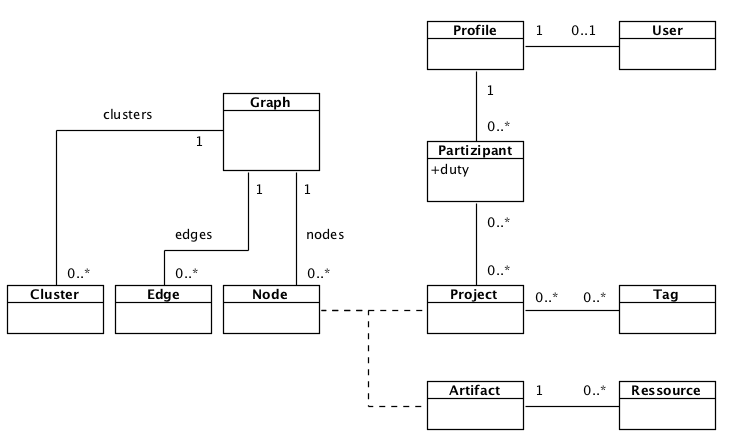
\includegraphics[width=1.0\textwidth]{img/models.png}  
   \caption{Ausgewählte Datenmodelle und ihre Assoziationen}
  \label{fig:models} 
\end{figure}

\section{Daten Modell für Graphen}
Ein Graph wurde als gerichteter Graph mit jeweils einer Liste für Knoten, Kanten und Cluster modelliert. Knoten und Kanten entsprechen denen aus der Graphentheorie bekannten Strukturen\footnote{Als konzeptionelle Referenz dient \cite[p.~531]{corman}}.  Cluster wurden eingeführt, um Nutzern die Möglichkeit zu geben, Knoten zu gruppieren und \tete{Tags} hinzuzufügen.

In der Datenbank sind für den \tete{Payload} eines Knotens nur Referenzen abgelegt. Der Payload beschreibt dabei den eigentlichen Inhalt eines Knotens, z.B. ein Projekt oder ein Artefakt. Wenn der Graph über die REST-Schnittstelle ausgeliefert wird, dann wird diese Payload-Referenz mit dem eigentlichen Inhalt des Knotens ersetzt. Dies verringert den Speicherbedarf des Graphs und verhindert das mehrfache Speichern des Payloads in der Datenbank.

\subsection{Versionierung}

Um die Veränderungen an einem Graph nachverfolgen zu können, wurde eine Versionierung für Graphen eingeführt. Dadurch, dass nur Referenzen auf den Inhalt eines Knotens gespeichert werden, ist die Größe eines Graphens vergleichsweise gering. Aus diesem Grund ist es möglich, alle Versionen eines Graphens in der Datenbank abzulegen. Zur Identifizierung bekommt ein Graph eine Gruppe (\tete{group}) zugewiesen. In einer Gruppe liegen die verschiedenen Versionen eines Graphen. Zusammen mit der Versionsnummer \tete{version}, welche bei jedem Update inkrementiert wird, bildet die Gruppe einen Schlüssel.

\subsection{Updaten eines Graphen}

Um ein Graphen-Update ausführen zu können, wurde die JSON Patch-Spezifikation\footnote{JavaScript Object Notation Patch \url{http://tools.ietf.org/html/rfc6902}} zur Veränderung von JSON-Objekten implementiert. Diese definiert eine JSON-Struktur, um ein gegebenes Objekt durch die Anwendung einer geordneten Folge von Änderungen in einen neuen Zustand zu überführen. Das Patch-Objekt ist ein JSON-Array, dessen Elemente als Operationen auf das zu verändernde JSON-Objekt angewendet werden sollen. Die definierten Operationen sind das Hinzufügen, Testen, Entfernen, Ersetzen, Verschieben und Kopieren von Attributen.

Alternativ bestünde die Möglichkeit, bei jeder Änderung den kompletten, geänderten Graphen zu senden. Da es sich hier um kleine Objekte handelt, wäre der Mehrbedarf an Bandbreite vertretbar. Für den Mehrnutzerbetrieb ist allerdings die Verwendung von JSON-Patch vorteilhaft, denn durch das explizite Senden der Änderungen ist ein Zusammenführen gleichzeitiger Änderungen von unterschiedlichen Quellen einfacher. Im Hinblick auf ebendiesen Vorteil wurde in Project-Zoom JSON-Patch verwendet.

\section{Datenmodell für Artefakte}

\tete{Artefakte} werden durch externe Konnektoren gefunden und anschließend durch den Backend-Core in der Datenbank abgelegt, wo alle Informationen enthalten sind, die charakteristisch für das jeweilige Artefakt sind. Eine Besonderheit zeigt sich im Feld \tete{metadata}. Hier können alle Informationen eines Connetors gespeichert werden, die keinem allgemeinen Feld zugeordnet werden können. Durch diese Speicherung von Informationen, die zwar im Moment für die Anwendung irrelevant sind und die nicht von allen Connectoren geliefert werden können, vermeidet man einen Informationsverlust. Bei der Weiterentwicklung der Anwendung können dann Informationen aus diesen Metadaten extrahiert und als eigenständige Felder verwendet werden. 

Zu einem Artefakt sind verschiedene \tete{Ressourcen} abgelegt. Eine Ressource bezieht sich hierbei auf die physikalische Repräsentation eines Artefakts. Das heißt, dass es zu jedem Ressourcenobjekt in der Datenbank eine zugehörige Datei im Dateisystem gibt. Beispielsweise ist die Originale Datei eine Ressource, generierte Thumbnails sind weitere. Das Feld \tete{typ} beschreibt die Art der Ressource und erlaubt einem Client die differenzierte Behandlung unterschiedlicher Typen.  

\section{Datenmodell für Nutzer}

Neben Artefakten können durch einen externen Connector auch Profile gesammelt werden. Diese Profile bestimmen die Zugriffsrechte eines Nutzers. Der mit einem Profil verknüpfte User enthält die Anmeldeinformationen, welche für das Authentifizierungsmodul SecureSocial benötigt werden. Ein User wird erst dann an ein Profil angehangen, wenn sich ein Nutzer mit der im Profil angegebenen E-Mail-Adresse für Project-Zoom registriert. Aus diesem Grund ist es auch nur Nutzern erlaubt sich zu registrieren, für die bereits ein Profil existiert.

\section{Zugriffsschutz für Datenbankobjekte}

Eine Anforderung der D-School bestand im Schutz der Daten. Dabei soll verhindert werden, dass Informationen aus Projekten für Personen, die kein Geheimhaltungsvertrag (NDA) für dieses Projekt unterschrieben haben, zugänglich sind. Studierende haben folglich nur Lesezugriff auf Projekte, an denen sie selbst teilgenommen haben oder die veröffentlicht\footnote{Aufgrund der fehlenden Einstellungsmöglichkeiten in der Filemaker Datenbank gibt es in der aktuellen Implementierung nicht die Möglichkeit ein Projekt als öffentlich zu kennzeichnen.} wurden. Schreibzugriff erhält ein Student nur als in der Filemaker-Datenbank vermerkter Teilnehmer des Projektes.

Bei der Betrachtung der Struktur von Zugriffsbeschränkungen fällt auf, dass diese abhängig von der zugriffssuchenden Person, der Art des Zugriffes und der Ressource sind. Basierend auf dieser Erkenntnis wurde ein sogenannter \tete{DBAccessContext} eingeführt. Für jeden Datenbankzugriff wird ein solcher Kontext benötigt. Mit Hilfe dessen können dann auf unterster Zugriffsebene, in den Funktionen \tete{insert}, \tete{update}, \tete{remove} und \tete{find}, die Berechtigungen überprüft werden.

Das Datenzugriffsobjekt für das jeweilige Datenmodell kann dann festlegen, wie mit Hilfe des DBAccessContext der Zugriff auf diese Methoden reguliert wird. Jedes dieser Datenzugriffsobjekte erbt von \tete{SecuredDAO}. In dieser Klasse findet die Ausführung der Datenbank Funktionen und die Zugriffsbeschränkung statt. Dadurch, dass die Zugriffsbeschränkungen für die jeweiligen Datenbankfunktionen einzeln festgelegt werden können, ist eine sehr feingranulare Differenzierung möglich.

Die Klasse \tete{SecuredDAO} überprüft die Berechtigungen wie folgt:
\begin{description}
\item[insert] Beim Hinzufügen wird direkt kontrolliert ob der User die Berechtigung hat, neue Elemente in das jeweilige Datenmodell einzufügen. Fehlt diese, wird die Aktion mit einem Fehler abgebrochen
\item[update] Ein Update Aktion benötigt immer eine Suchanfrage und das eigentliche Update was auf die gefundenen Ergebnisse angewandt wird. Soll ein User nicht alle Objekte updaten können, so wird an die Suchanfrage die jeweilige Einschränkung angehangen. Damit wird verhindert, dass Objekte gefunden werden, auf die der User keinen Zugriff hat. Objekte die nicht gefunden werden, können demnach auch nicht verändert werden.
\item[find, remove] Für das Abfragen und Löschen ist eine Suchanfrage notwendig. Diese wird genauso verändert wie dies für die \tete{update}-Funktion beschrieben ist. Der Ergebnisraum wird somit schon während der Abfrage auf die dem User zugänglichen Objekte beschränkt.
\end{description}
